%\section{System Dynamics in Fair Operation}\label{sec:aggregation:performance_model:analytical_model}

%\subsubsection*{System Model}\label{sec:network:performance_model:analytical_model:system_model}


\subsection{The Case of Two Systems}\label{sec:aggregation:performance_model:analytical_model:2_systems}

% \begin{figure}[htb!]
% 	\centering
%  	\includegraphics[width=0.66\textwidth]{figures/sysmodel3}
%   	\caption{System model.}
%   	\label{fig:sysmodel}
% \end{figure}


We first consider a scenario with two different Internet access links. %Figure~\ref{fig:sysmodel} shows a schematic view of the model as described above and highlights the most important system characteristics.
In the case of two links, the actual system state can be described by two random variables $X_1$ and $X_2$, which represent the number of occupied bandwidth fractions in the respective access link. As the model components comprise the memoryless property, a two-dimensional Markov process can be analyzed using standard techniques of queueing theory.

With the state probabilities
\begin{equation}
x(i,j) = P(X_1=i, X_2=j),\ 0\leq i\leq n_1, 0\leq j \leq n_2,
\end{equation}
i.e., the probability that $i$ bandwidth fractions are occupied in system 1 and $j$ bandwidth fractions are occupied in system 2, the two-dimensional state transition diagram, presented in Figure~\ref{fig:statetransitions}, can be arranged. Two major areas are visible. In the upper left part and the lower right part (white background), each system operates independently in such way that all arriving requests are served locally by this system. In the top-right and bottom-left parts (shaded in gray), one of the links is in offloading state and the other link is in support state. In these cases, all traffic arriving at the offloading link will be served by the supporting link. Thus, blocking only occurs when the other link cannot help, i.e., in states $\{(n_1,j) : \lfloor\alpha_2 n_2\rfloor \leq j \leq n_2\}$ and $\{(i,n_2) : \lfloor\alpha_1 n_1\rfloor\leq i \leq n_1\}$.

\begin{figure*}[tb]
	\centering
 	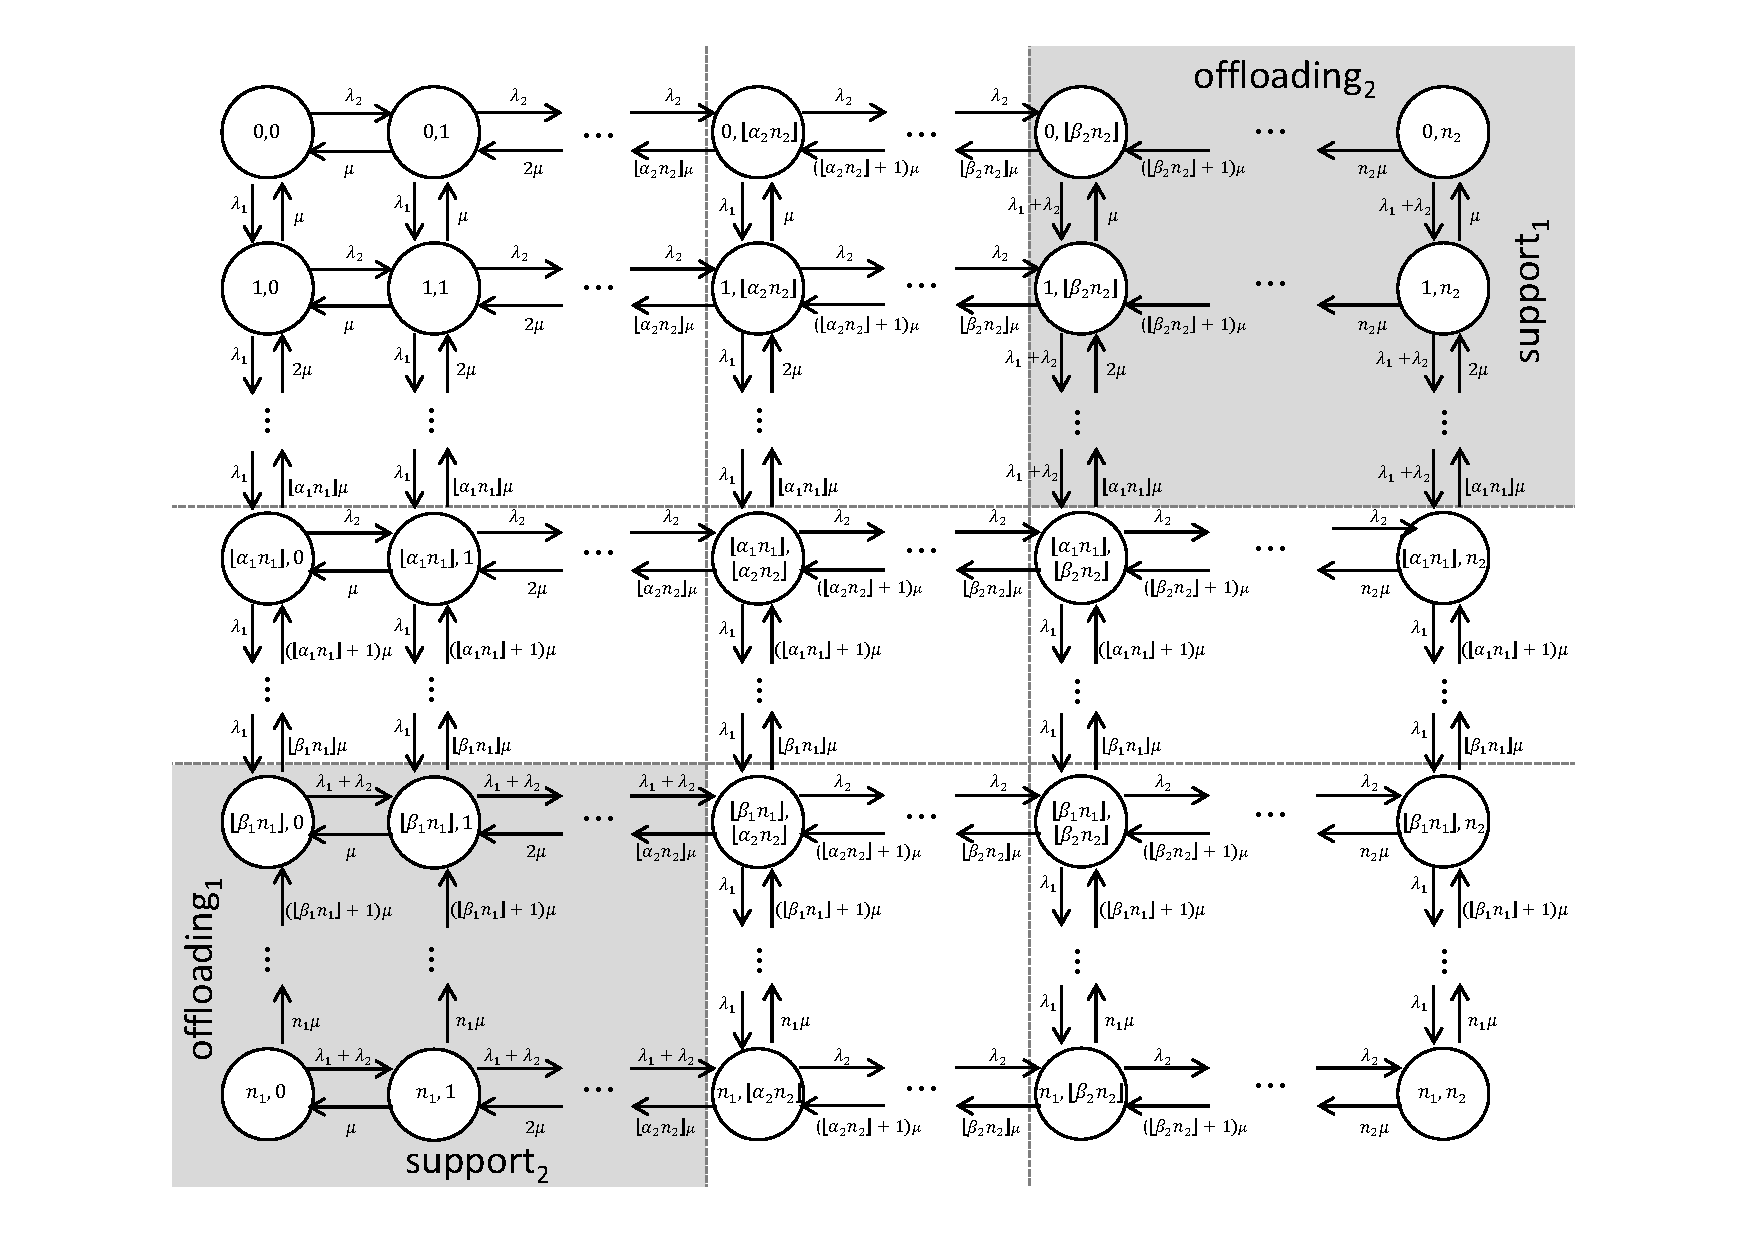
\includegraphics[width=1.0\textwidth]{aggregation/performance_model/figures/states}
  	\caption{The state transition diagram.}
  	\label{fig:statetransitions}
\end{figure*}

The blocking probability is calculated by

\begin{equation}
  p_b =
\end{equation}

\subsection{The Case of Multiple Systems}\label{sec:aggregation:performance_model:analytical_model:m_systems}

The case, in which $m$ Internet access links offload traffic according to the policy defined via the support and offloading thresholds, is more interesting, since much more than two access links can be available in densely populated neighborhoods and since the potential of the approach increases with the number of links available for bandwidth sharing.
We start with assuming that all access links are equal ($n=n_i, \forall i\in\{1,\ldots,m\}$) and face equal loads ($\lambda=\lambda_i, \forall i\in\{1,\ldots,m\}$) and policies ($\alpha = \alpha_i, \beta = \beta_i, \forall i\in\{1,\ldots,m\}$). First, we distinguish one access link, and merge the remaining $m-1$ cooperating access links into a composite system. This reduces the problem of $m$ systems to two systems. Still, the complexity of the composite system prohibits creating and analyzing the two-dimensional state transition diagram as it was done in \cite{burger2016phycom}. Thus, we apply a fixed point approach to analyze this system.%, which is presented in Figure~\ref{fig:composite}.
Therefore, we model an observed system, which will take into account offloading to and supporting the abstract composite system. For simplifying the notation, we define the macro state probabilities $p_1$ (support), $p_2$ (normal), and $p_3$ (offload):

\begin{align}
\begin{split}
p_1 &= \sum x(i),  0 \leq i < \lfloor\alpha\cdot n\rfloor \\
p_2 &= \sum x(i), \lfloor\alpha\cdot n\rfloor\leq i < \lfloor\beta\cdot n\rfloor \\
p_3 &= \sum x(i), \lfloor\beta\cdot n\rfloor \leq i \leq n
\end{split}
\label{eq:macro}
\end{align}

In the support macro state, the arrival rate will be increased by $\lambda_s$, i.e., the arrivals that are offloaded by the composite system. $\lambda_s$ can be computed as shown in Equation~\ref{eq:lambda_s} from the multinomial probability that $j$ of the $m-1$ links in the composite system are in offloading state, and $k$ links in the composite system can support.

\small
\begin{equation}
\lambda_{s} = \sum_{j=1}^{m-1}\sum_{k=0}^{m-1-j} \binom{m-1}{j}\binom{m-j-1}{k}p^j_3 p^k_1 p_2^{m-j-k-1}\frac{j\lambda}{k+1}
\label{eq:lambda_s}
\end{equation}
\normalsize

The arrival rate is decreased by $\lambda_o$ in the offloading macro state when the composite system can support the observed system, i.e., at least one of the $m-1$ systems is in support macro state.

\begin{equation}
\lambda_{o} = (1-(1-p_1)^{m-1})\lambda
\end{equation}

This gives new steady state equations for the observed system as described in Equation~\ref{eq:iteration}. As all access links have equal load, and thus, show a homogeneous behavior, not only the state probabilities of the observed system, but also of the $m-1$ systems in the composite system are influenced. Thus, the state probabilities of all $m$ links can be obtained by computing the state probabilities of the observed system. Therefore, we initialize the observed system with equal state probabilities. Then, we iterate the offloading and support and normalize the state probabilities  until a fixed point is reached.

\begin{align}
\begin{split}
&x(i)=
\begin{cases}
\frac{x(i-1)(\lambda+\lambda_s)}{i\cdot\mu}, &0\leq i < \lfloor\alpha\cdot n\rfloor \\
\frac{x(i-1)\lambda}{i\cdot\mu}, &\lfloor\alpha\cdot n\rfloor\leq i < \lfloor\beta\cdot n\rfloor \\
\frac{x(i-1)(\lambda-\lambda_o)}{i\cdot\mu}, &\lfloor\beta\cdot n\rfloor \leq i \leq n \\
\end{cases}\\
&\sum_{i=0}^n x(i) = 1
\end{split}
\label{eq:iteration}
\end{align}

For our modeled bandwidth aggregation system with $m$ Internet access links, we consider the blocking probability $p_{b} = x(n)\cdot (1-p_1)^{m-1}$ of a link, which is calculated by the probability that a request arrives when the link is fully loaded (i.e., in state $n$) and none of the $m-1$ other links can support.

Moreover, we take a look at the received bandwidth at each access link $E[X_{A_i}]$. Thereby, $X_{A_i}$ is a random variable for the number of bandwidth fractions (in all systems), which are occupied by arrivals from system $i$. It is obvious that $E[X_{A_i}] = E_0[X_i]$ for the partitioned system. In case of offloading between $m$ equal links, $E[X_{A_i}]= \frac{\lambda}{\mu}\cdot (1-p_{b})$ is equal for all links and can be calculated from the mean total number of occupied bandwidth fractions by taking into account the share of accepted requests.
Finally, we also quantify the percentage of bandwidth gain for each system as
\begin{equation}
\omega_i = \frac{E[X_{A_i}]-E_0[X_i]}{E_0[X_i]}\, .
\end{equation}
